\documentclass[aspectratio=169]{beamer}

% Setup
% Thesis Team Setup - Custom Setup for Candidate, Supervisor, Co-Supervisors in Beamer
% Place this file in your project directory and \input{thesis_team_setup.tex} in your main .tex

% Required packages
\usepackage{tabularx}
\usepackage[british]{babel}
\usepackage[utf8]{inputenc}
\usepackage{graphicx,hyperref,ru,url}
\usepackage{lmodern,tabularx,background,tikz}
\usepackage{scrextend}
\usepackage[skip=2pt]{caption}
\usepackage{subcaption}
\usepackage{xcolor}
\usepackage{fontawesome5}
\usepackage{tcolorbox}
\usepackage{tikz}
\usepackage{mdwlist}

% Bibliography setup for [Author, et al., Year] format
\usepackage[style=authoryear,backend=biber,maxcitenames=1,mincitenames=1]{biblatex}
\addbibresource{references.bib}
\usetikzlibrary{positioning,arrows.meta,calc,automata,decorations.pathreplacing}
\tikzset{
  accepting/.style={circle, draw, double, minimum size=7mm}
}

% Team member macros (LaTeX2e, needs \makeatletter...\makeatother)
\makeatletter
\newcommand{\candidate}[1]{\def\@candidate{#1}}
\newcommand{\supervisor}[1]{\def\@supervisor{#1}}
\newcommand{\cosupervisors}[1]{\def\@cosupervisors{#1}}
\newcommand{\printthesisteam}{
  \vspace{0.3cm}
  \begin{center}
    \begin{tabular}{@{}p{0.28\linewidth}@{\hspace{0.05\linewidth}}p{0.28\linewidth}@{\hspace{0.05\linewidth}}p{0.35\linewidth}@{}}
      \raggedright\footnotesize \textbf{Candidate}: \@candidate &
      \centering\footnotesize \textbf{Supervisor}: \@supervisor &
      \raggedleft\footnotesize \textbf{Co-Supervisor}: \@cosupervisors \\
    \end{tabular}
  \end{center}
}
\makeatother

% Title and metadata
\title[RU style for Beamer]{A New Compression Technique for Repetitive Tries}
\author[Davide Tonetto]{\changefontsizes{12pt} \textsc{Davide Tonetto}}
\institute[Ca' Foscari]{
\changefontsizes{10pt}
  \textsc{Ca’ Foscari University of Venice \\
Department of Environmental Sciences, Informatics and Statistics}
}
\date[master thesis]{
{\changefontsizes{14pt}
  \textsc{Master's Thesis Defense} \\[0.3cm] \changefontsizes{8pt}
  Computer Science and Information Technology\\[-0.5em] \textit{Artificial Intelligence and Data Engineering} }\\[0.5cm]
  \textsc{6th November 2025}
  \printthesisteam
}

% Watermark background (logo on right, faint, scaled, shifted)
\setbeamertemplate{background}{
  \begin{tikzpicture}[remember picture,overlay]
    \node[anchor=east, opacity=0.05, scale=0.9, yshift=-0.72cm] at ([xshift=3.3cm]current page.east) 
      {\includegraphics[height=0.8\paperheight]{UNIVE_square_black.png}};
  \end{tikzpicture}
}

\newcommand{\fancysectionframe}[2][]{%
  \begin{frame}[plain]
    \centering
    \vfill
    {\color{rured} \bfseries \LARGE #2}
    \ifx&#1&\else
      \\[0.5em]
      {\color{black} \large #1}
    \fi
    \par\vspace{0.5ex}
    {\color{rured}\rule{0.45\paperwidth}{1.7pt}}
    \vfill
  \end{frame}
}

% Palette di colori ad alta visibilità e colorblind-safe (Okabe–Ito)
\definecolor{oiBlue}{HTML}{0072B2}
\definecolor{oiSkyBlue}{HTML}{56B4E9}
\definecolor{oiOrange}{HTML}{E69F00}
\definecolor{oiGreen}{HTML}{009E73}
\definecolor{oiVermillion}{HTML}{D55E00}
\definecolor{oiPurple}{HTML}{CC79A7}
\definecolor{oiLightGrey}{HTML}{D3D3D3}
\definecolor{oiRed}{HTML}{FF0000}

\newenvironment{greenblock}[1]{%
  \setbeamercolor{block title}{bg=green!40!black, fg=white}%
  \setbeamercolor{block body}{bg=green!10!white, fg=black}%
  \begin{block}{#1}}{\end{block}}

\setbeamertemplate{caption}[numbered]

% Setup thesis team members
\candidate{Davide Tonetto}
\supervisor{Nicola Prezza}
\cosupervisors{Alessio Campanelli}



\begin{document}

\begin{frame}[plain]
  \titlepage
\end{frame}

% \begin{frame}
%   \frametitle{Outline}
%   \tableofcontents
% \end{frame}

\fancysectionframe{Introduction and Motivation}

\section{Introduction and Motivation}
\begin{frame}{Motivation}
  \begin{itemize}
    \item Tries are fundamental data structures for representing large sets of strings.
    \item Efficient for prefix-based queries, but often very large in memory.
    \item Typical applications:
      \begin{itemize}
        \item Autocomplete and predictive text
        \item Spell checking
        \item IP routing
        \item Bioinformatics (DNA pattern matching)
      \end{itemize}
    \item Objective: reduce memory footprint while keeping efficient queries.
  \end{itemize}
\end{frame}

\begin{frame}{Example: Trie Representation}
\centering
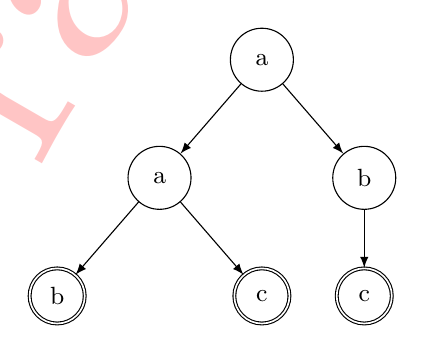
\begin{tikzpicture}[
  every node/.style={draw, circle, minimum size=8mm, inner sep=0pt, font=\small},
  edge from parent/.style={draw, -latex},
  level distance=1.5cm,
  sibling distance=2.6cm
  ]

% Root is 'a'
\node (a) {a}
  child {node {a}
    child {node[accepting] {b} [label=right:{word "aab"}]}
    child {node[accepting] {c} [label=right:{word "aac"}]}
  }
  child {node {b}
    child {node[accepting] {c} [label=right:{word "abc"}]}
  };

\end{tikzpicture}

\vspace{0.3cm}
\small
Each path from the root node \texttt{a} to a leaf represents one string in the language 
$\{aab, aac, abc\}$.
\end{frame}

\begin{frame}{Challenges}
  \begin{itemize}
    \item Tries can contain large, identical subtrees.
    \item Standard compression (e.g., XBWT, LZ77, top tree) does not exploit structural repetitions.
  \end{itemize}

  \vspace{0.3cm}
  Fundamental trade-off between compression and indexability:
      \begin{itemize}
        \item \textbf{Full Indexability, No Compression:} the input trie itself can be used as an index. It offers no compression, as even highly repetitive subtrees are stored explicitly
        \item \textbf{Full Compression, Difficult Indexing:} maximum compression but very poor indexability.
      \end{itemize}
  \textbf{Goal:} find the sweet spot between these two extremes.
\end{frame}

% === THEORY BACKGROUND ===
\fancysectionframe{Theoretical Background}

\section{Theoretical Background}
\begin{frame}{Tries, DFAs and Minimization}
  \begin{itemize}
    \item A trie can be seen as an \textbf{acyclic DFA}.
    \item Minimizing a DFA merges \textbf{Myhill–Nerode equivalent states}.
    \item Revuz’ algorithm allows linear-time minimization for acyclic DFAs.
  \end{itemize}
  \centering
  %\includegraphics[width=0.7\textwidth]{fig_revuz_example.png}
  \small
  Example: reduction of an acyclic DFA by merging equivalent subtrees.
\end{frame}

\begin{frame}{XBWT (Extended Burrows–Wheeler Transform)}
  \begin{itemize}
    \item Extends the classic BWT from strings to labeled trees.
    \item Encodes the tree as two arrays:
      \begin{itemize}
        \item $S_\alpha$: node labels
        \item $S_{last}$: structure bits
      \end{itemize}
    \item Enables compressed storage and prefix queries.
  \end{itemize}
  \centering
  % \includegraphics[width=0.8\textwidth]{fig_xbwt_example.png}
  \small
  The children of each node form a contiguous block in $S_\alpha$.
\end{frame}

% === PROPOSED METHOD ===
\fancysectionframe{Proposed Compression Scheme}

\section{Proposed Compression Scheme}
\begin{frame}{Motivation for a New Approach}
  \begin{itemize}
    \item Full minimization $\Rightarrow$ excellent compression but unindexable.
    \item Uncompressed trie $\Rightarrow$ fully indexable but memory-hungry.
  \end{itemize}
  
  \vspace{0.3cm}
  Our approach:
      \begin{block}{Partial Minimization}
      Produce a smaller automaton that remains indexable
      by allowing partial merging of equivalent subtrees.
      \end{block}
  Key concept: \textbf{p–sortable automata}.
\end{frame}

\begin{frame}{p–Sortable Automata}

\begin{block}{p–sortable Automaton}
  Let $\mathcal{A} = (Q, \Sigma, \delta, q_0, F)$ be a finite-state automaton. We call $\mathcal{A}$ \emph{$p$--sortable} if there exists a co--lexicographic order $\leq$ on $Q$ such that $Q$ can be partitioned into $p$ chains $\{Q_i\}_{i=1}^p$, where each $(Q_i, \leq)$ is totally ordered.
\end{block}

Let $\mathcal{A}$ be a $p$--sortable automaton. There exists a compressed data structure for $A$ that supports subpath queries on a query word $\alpha$ of length $m$ in $O(mp^2\log\log(p|\Sigma|))$ time. The space required is:
\begin{itemize}
  \item $\log(|\Sigma|) + \log p + 2$ bits per edge if $A$ is a DFA.
  \item $\log(|\Sigma|) + 2\log p + 2$ bits per edge if $A$ is an NFA.
\end{itemize}

\end{frame}

\begin{frame}{The Intuition}
  \begin{itemize}
    \item Parameter $p$ interpolates between the two extremes:
      \begin{itemize}
        \item $p=1$: Wheeler graph $\Rightarrow$ maximum indexability, less compression.
        \item $p \to \infty$: more compression, less indexability.
      \end{itemize}
    \item Increasing $p$ improves compression but complicates indexing.
  \end{itemize}
  \vspace{0.3cm}
  \centering
  % \includegraphics[width=0.65\textwidth]{fig_psortable_graph.png}
  \small
  Example of a 2–sortable automaton: partial merging with preserved order.
\end{frame}

\begin{frame}{Compression Pipeline}
  \begin{enumerate}
    \item Sort nodes by co–lexicographic order.
    \item Partition nodes into $p$ subsequences respecting the order.
    \item Merge consecutive Myhill–Nerode equivalent states within each partition.
    \item Construct the resulting compressed p–sortable automaton.
  \end{enumerate}
  \centering
  % \includegraphics[width=0.8\textwidth]{fig_pipeline_scheme.png}
\end{frame}

\begin{frame}{String Partitioning Problem}
  Consider a sting $s$.
  \begin{block}{Run}
  Maximal contiguous subsequence of identical symbols within $s$. 
  \end{block}
  \begin{block}{String Partitioning Problem}
  Partition $s$ into $p$ subsequences minimizing number of runs. 
  \end{block}
  \centering
  % \includegraphics[width=0.7\textwidth]{fig_string_partitioning_example.png}
\end{frame}

\begin{frame}{Example: String Partitioning Problem}
\small 

\[
s = \texttt{2213122152}
\]
of length 10.  
The number of runs in $S$ is 8, given by the decomposition:
\[
\texttt{(22)(1)(3)(1)(22)(1)(5)(2)}
\]

A possible partition is:
\begin{itemize}
  \item $I_1 = \{3, 5, 8, 9\}$
  \item $I_2 = \{1, 2, 4, 6, 7, 10\}$
\end{itemize}

This yields the following subsequences:
\begin{itemize}
  \item $S[I_1] = \texttt{1115}$  
        $\Rightarrow$ 2 runs: $(\texttt{111})$, $(\texttt{5})$
  \item $S[I_2] = \texttt{223222}$  
        $\Rightarrow$ 3 runs: $(\texttt{22})$, $(\texttt{3})$, $(\texttt{222})$
\end{itemize}

\textbf{Total runs:} $2 + 3 = 5$  
$\Rightarrow$ reduction from the original 8 runs in $S$.
\end{frame}

\begin{frame}{Reduction to Bipartite Graph Matching}
  \begin{itemize}
    \item The String Partitioning Problem can be reduced to:
      \[
        \text{Minimum Weight Perfect Bipartite Matching (MWPBM)}
      \]
    \item Nodes correspond to string characters; edges encode run boundaries cost between characters.
    \item Allows to use efficient, well-studied algorithms to find the optimal solution.
  \end{itemize}
\end{frame}

\begin{frame}{Example: Min-Weight Bipartite Graph Matching}
  \centering
  \centering
  \begin{figure}[H]
    \centering
    \tikzset{main/.style = {draw, circle, thick, minimum size=8mm, inner sep=0pt}}
    \begin{subfigure}[b]{0.3\textwidth}
        \centering
        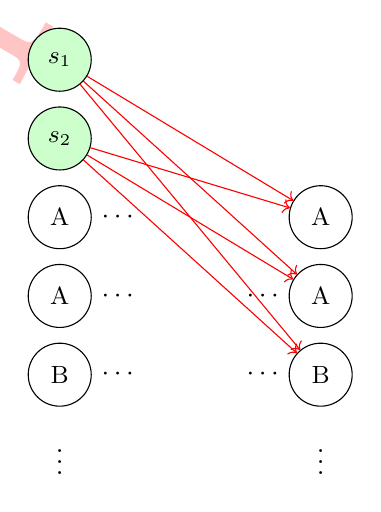
\begin{tikzpicture}[node distance=10mm, auto=center]
            \tikzstyle{main} = [circle, draw, minimum size=0.8cm, font=\small]
            \tikzstyle{source} = [circle, draw, minimum size=0.8cm, font=\small, fill=green!20]
            \tikzstyle{dest} = [circle, draw, minimum size=0.8cm, font=\small, fill=blue!20]
            
            % Left column (sources)
            \node[source] (1s) {$s_1$};
            \node[source] (2s) [below of=1s] {$s_2$};
            \node[main] (3s) [below of=2s] {A};
            \node[right=0cm of 3s] {$\cdots$};
            \node[main] (4s) [below of=3s] {A};
            \node[right=0cm of 4s] {$\cdots$};
            \node[main] (5s) [below of=4s] {B};
            \node[right=0cm of 5s] {$\cdots$};
            \node (dots_s) [below of=5s] {\vdots}; % Vertical dots

            % Right column (destinations)
            \node[main] (1d) [right=2.5cm of 3s] {A};
            \node[main] (2d) [below of=1d] {A};
            \node[left=0cm of 2d] {$\cdots$};
            \node[main] (3d) [below of=2d] {B};
            \node[left=0cm of 3d] {$\cdots$};
            \node (dots_d) [below of=3d] {\vdots}; % Vertical dots

            % Arrows
            \draw[red, ->] (1s) -- (1d);
            \draw[red, ->] (1s) -- (2d);
            \draw[red, ->] (1s) -- (3d);
            \draw[red, ->] (2s) -- (1d);
            \draw[red, ->] (2s) -- (2d);
            \draw[red, ->] (2s) -- (3d);
        \end{tikzpicture}
        \caption{}
        \label{fig:sub1}
    \end{subfigure}
    \hfill % Space between subfigures
    \tikzset{main/.style = {draw, circle, thick, minimum size=8mm, inner sep=0pt}}
    \begin{subfigure}[b]{0.3\textwidth}
        \centering
        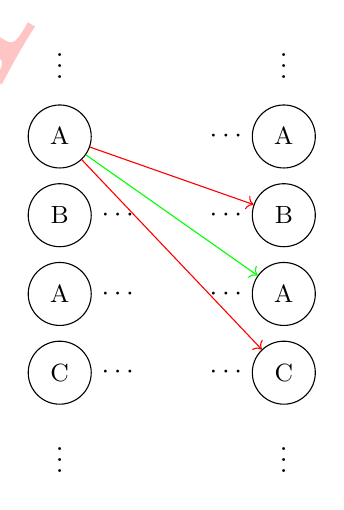
\begin{tikzpicture}[node distance=10mm, auto=center]
            \tikzstyle{main} = [circle, draw, minimum size=0.8cm, font=\small]
            \tikzstyle{source} = [circle, draw, minimum size=0.8cm, font=\small, fill=green!20]
            \tikzstyle{dest} = [circle, draw, minimum size=0.8cm, font=\small, fill=blue!20]

            % Left column (tree nodes)
            \node (dots_s_top) {\vdots};
            \node[main] (3s) [below of=dots_s_top] {A};
            \node[main] (4s) [below of=3s] {B};
            \node[right=0cm of 4s] {$\cdots$};
            \node[main] (5s) [below of=4s] {A};
            \node[right=0cm of 5s] {$\cdots$};
            \node[main] (6s) [below of=5s] {C};
            \node[right=0cm of 6s] {$\cdots$};
            \node (dots_s_bottom) [below of=6s] {\vdots};

            % Right column (destinations)
            \node (dots_d_top) [right=2.5cm of dots_s_top] {\vdots};
            \node[main] (1d) [below of=dots_d_top] {A};
            \node[left=0cm of 1d] {$\cdots$};
            \node[main] (2d) [below of=1d] {B};
            \node[left=0cm of 2d] {$\cdots$};
            \node[main] (3d) [below of=2d] {A};
            \node[left=0cm of 3d] {$\cdots$};
            \node[main] (4d) [below of=3d] {C};
            \node[left=0cm of 4d] {$\cdots$};
            \node (dots_d_bottom) [below of=4d] {\vdots};

            % Arrows
            \draw[red, ->] (3s) -- (2d);
            \draw[red, ->] (3s) -- (4d);
            \draw[green, ->] (3s) -- (3d);
        \end{tikzpicture}
        \caption{}
        \label{fig:sub2}
    \end{subfigure}
    \hfill % Space between subfigures
    \tikzset{main/.style = {draw, circle, thick, minimum size=8mm, inner sep=0pt}}
    \begin{subfigure}[b]{0.3\textwidth}
        \centering
        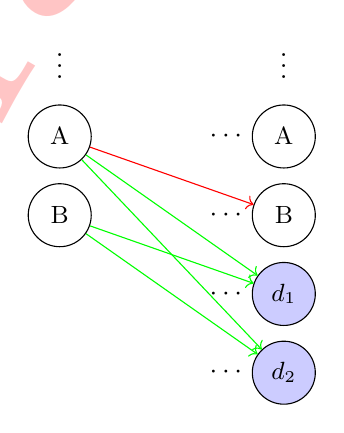
\begin{tikzpicture}[node distance=10mm, auto=center]
            \tikzstyle{main} = [circle, draw, minimum size=0.8cm, font=\small]
            \tikzstyle{source} = [circle, draw, minimum size=0.8cm, font=\small, fill=green!20]
            \tikzstyle{dest} = [circle, draw, minimum size=0.8cm, font=\small, fill=blue!20]

            % Left column (original destinations)
            \node (dots_s_top) {\vdots};
            \node[main] (7s) [below of=dots_s_top] {A};
            \node[main] (9s) [below of=7s] {B};

            % Right column (bipartite graph destinations)
            \node (dots_d_top) [right=2.5cm of dots_s_top] {\vdots};
            \node[main] (5d) [below of=dots_d_top] {A};
            \node[left=0cm of 5d] {$\cdots$};
            \node[main] (6d) [below of=5d] {B};
            \node[left=0cm of 6d] {$\cdots$};
            \node[dest] (8d) [below of=6d] {$d_1$};
            \node[left=0cm of 8d] {$\cdots$};
            \node[dest] (9d) [below of=8d] {$d_2$};
            \node[left=0cm of 9d] {$\cdots$};

            % Arrows
            \draw[red, ->] (7s) -- (6d);
            \draw[green, ->] (7s) -- (8d);
            \draw[green, ->] (7s) -- (9d);
            \draw[green, ->] (9s) -- (8d);
            \draw[green, ->] (9s) -- (9d);
        \end{tikzpicture}
        \caption{}
        \label{fig:sub3}
    \end{subfigure}
    \label{fig:reduction_small_examples}
  \end{figure}
\end{frame}

% === IMPLEMENTATION AND RESULTS ===
\fancysectionframe{Implementation and Experiments}

\section{Implementation and Experiments}
\begin{frame}{Experimental setup}
  \begin{itemize}
    \item Implemented in \textbf{C++} for performance.
    \item \textbf{CPU and RAM}: Apple M4 Pro, 24 GB.
    \item \textbf{Dataset}: synthetic generated tries to control repetitiveness.
  \end{itemize}
\end{frame}

\begin{frame}{Experimental Results}
  \begin{itemize}
    \item Increasing $p$ from 1 to 2 halves the number of states.
    \item Compression ratio improves rapidly, approaching the minimal number of states for larger $p$.
  \end{itemize}
  \centering
  \includegraphics[width=0.9\textwidth]{img/tree_compression_analysis_high_a.pdf}
\end{frame}

\begin{frame}{Experimental Results}
  \centering
  \includegraphics[width=1\textwidth]{img/tree_compression_analysis_high_b.pdf}
\end{frame}

% === CONCLUSIONS ===
\fancysectionframe{Conclusions}

\section{Conclusions}
\begin{frame}{Conclusions}
  \begin{itemize}
    \item Proposed a new trie compression method based on p–sortable automata.
    \item Achieves:
      \begin{itemize}
        \item Significant memory reduction on repetitive data.
        \item Efficient querying capability.
        \item Flexibility via parameter $p$.
      \end{itemize}
    \item Opens new directions for compressed automata and string indexing.
  \end{itemize}
\end{frame}

\begin{frame}{Future Work}
  \begin{itemize}
    \item \textbf{Scalability}: Investigate improvements to the proposed reduction for the String Partitioning problem to develop more scalable and efficient solutions for large-scale applications.
	  \item \textbf{DFA Construction}: Explore methods to directly construct a $p$—sortable deterministic finite automaton from the pipeline, potentially by developing a pruning strategy for the output NFA.
	  \item \textbf{DFA Minimization}: Minimize the size of the returned automaton, potentially by providing explicit guarantees of minimality of the returned $p$—sortable DFA.
  \end{itemize}
\end{frame}

\end{document}